\section*{Part D}
\addcontentsline{toc}{section}{Part D}

\begin{tcolorbox}
  D.1) Synthesise and plot this square wave (provide your Matlab code as well). Calculate the percentage overshoot of the synthesised waveform (compared with the ideal waveform) at the discontinuity. How does this compare with the expected limit of 17.9\%?
\end{tcolorbox}

\lstinputlisting[
  caption = Requirement 4 MATLAB code,
  label = code:D_r_1,
]{matlab/D_r_1.m}

\begin{figure}[htbp]
  \centering
  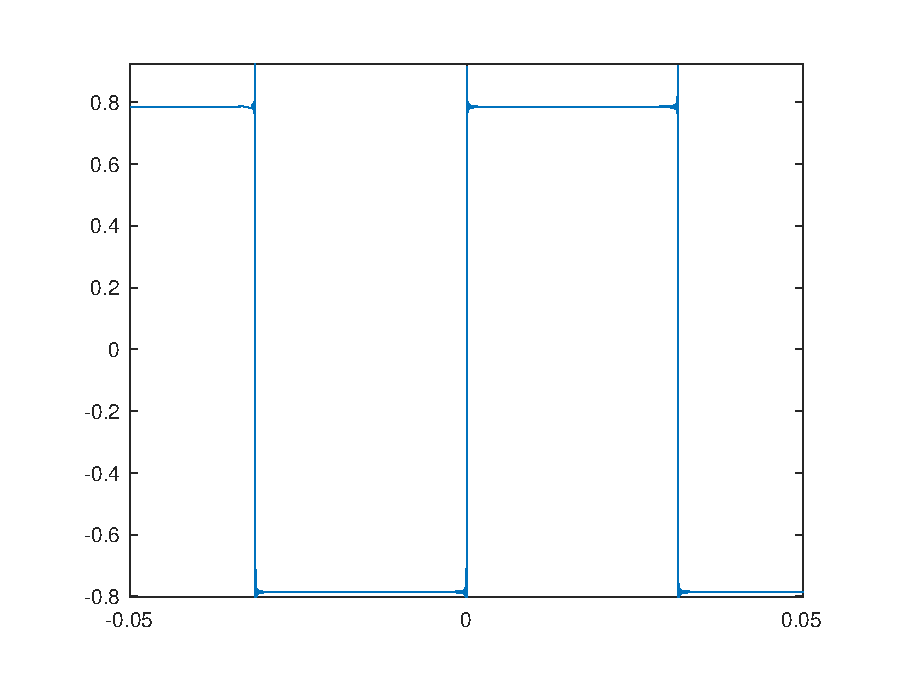
\includegraphics [width=2in]{matlab/fig/D_r_1.eps}
  \caption{synthesised square wave}    
  \label{fig:D_r_1}
\end{figure}

\begin{figure}[htbp]
  \centering
  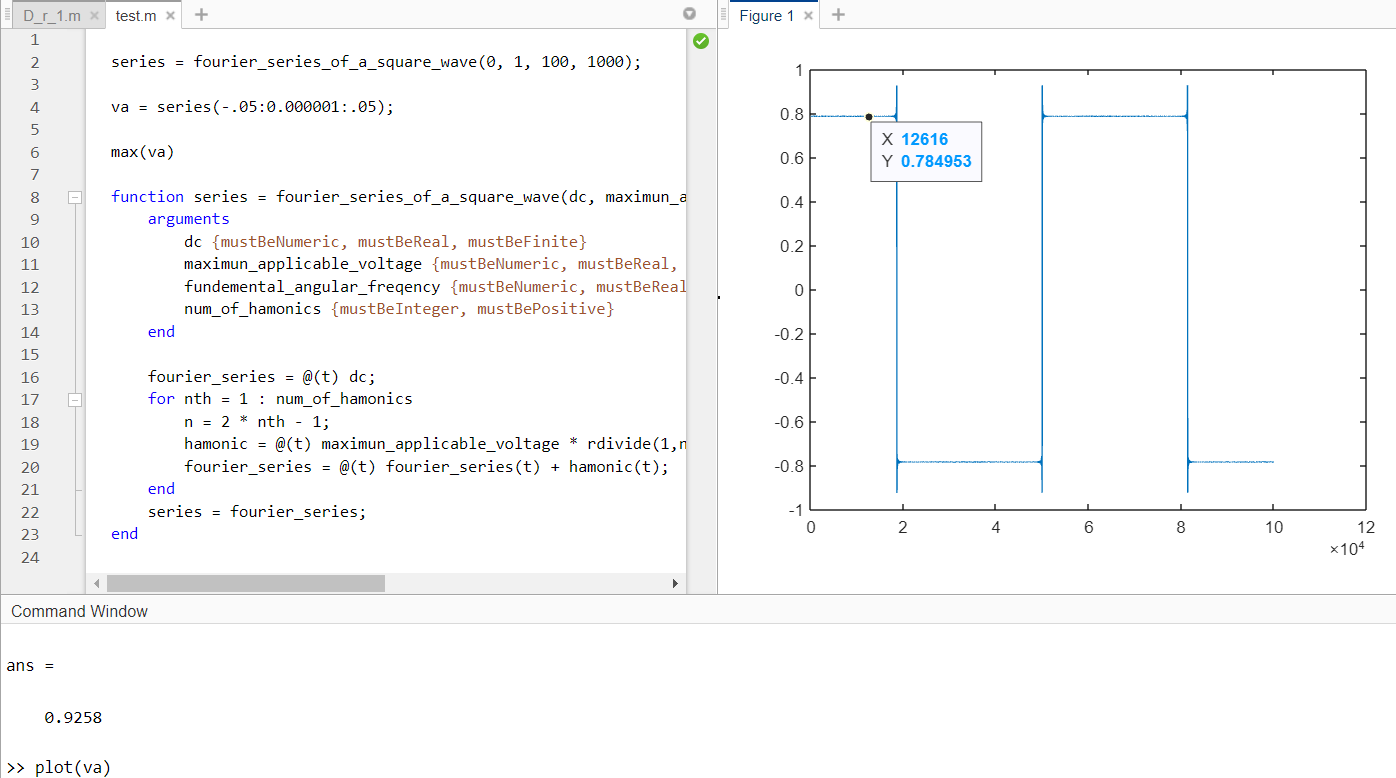
\includegraphics [width=\textwidth]{matlab/fig/D_r_1_2.png}
  \caption{overshoot value}    
  \label{fig:D_r_1_2}
\end{figure}

\[ \textit{percentage overshoot} = \frac{0.9258 - 0.7650}{0.7650} \times 100\% = 21.02 \% \]

21.02\% is greater than the expected limit of 17.9\%.

\begin{tcolorbox}
  D.2) What is the name of this overshoot? Explain it.
\end{tcolorbox}

This overshoot is called Gibbs phenomenon. This phenomenon describes summing a finite Fourier series for a discontinuous signal will end up with overshoots at each discontinuous part. These overshoots will not be eliminated by increasing the number of hamonics used for approximation.

\begin{tcolorbox}
  D.3) (a) Give the Fourier series for the resulting waveform if the above square wave is used as an input for a low-pass filter with gain and phase responses as given in Figures 8 and 10 respectively.
\end{tcolorbox}

\[ \frac{3}{\pi}\Big( - \cos(2\pi f_o t) + \frac{1}{3}\cos(2\pi 3f_o t) - \frac{1}{5}\cos(2\pi 5f_o t) + \frac{1}{7}\cos(2\pi 7f_o t) - \frac{1}{9}\cos(2\pi 9f_o t)\Big) \]

\begin{tcolorbox}
  D.3) (b) Give the Fourier series for the resulting waveform if the above square wave is used as an input for a low-pass filter with gain and phase responses as given in Figures 8 and 11 respectively.
\end{tcolorbox}

\[ \frac{3}{\pi}\Big( - \cos(2\pi f_o t) - \frac{1}{3}\cos(2\pi 3f_o t) - \frac{1}{5}\cos(2\pi 5f_o t) - \frac{1}{7}\cos(2\pi 7f_o t) - \frac{1}{9}\cos(2\pi 9f_o t)\Big) \]

\begin{tcolorbox}
  D.3) (c) Give the Fourier series for the resulting waveform if the above square wave is used as an input for a band-pass filter with gain and phase responses as given in Figures 9 and 10 respectively.
\end{tcolorbox}

\[ \frac{3}{\pi}\Big(\frac{1}{2} \times \frac{1}{3}\cos(2\pi 3f_o t) - \frac{1}{5}\cos(2\pi 5f_o t) + \frac{1}{7}\cos(2\pi 7f_o t) - \frac{1}{2} \times \frac{1}{9}\cos(2\pi 9f_o t)\Big) \]

\begin{tcolorbox}
  D.4) Synthesise the above waveforms and draw the obtained waveforms for filters (a), (b) and (c), providing the Matlab code as well.
\end{tcolorbox}

\lstinputlisting[
  caption = Requirement 4 MATLAB code,
  label = code:D_r_4,
]{matlab/D_r_4.m}

\begin{figure}[htbp]
  \centering
  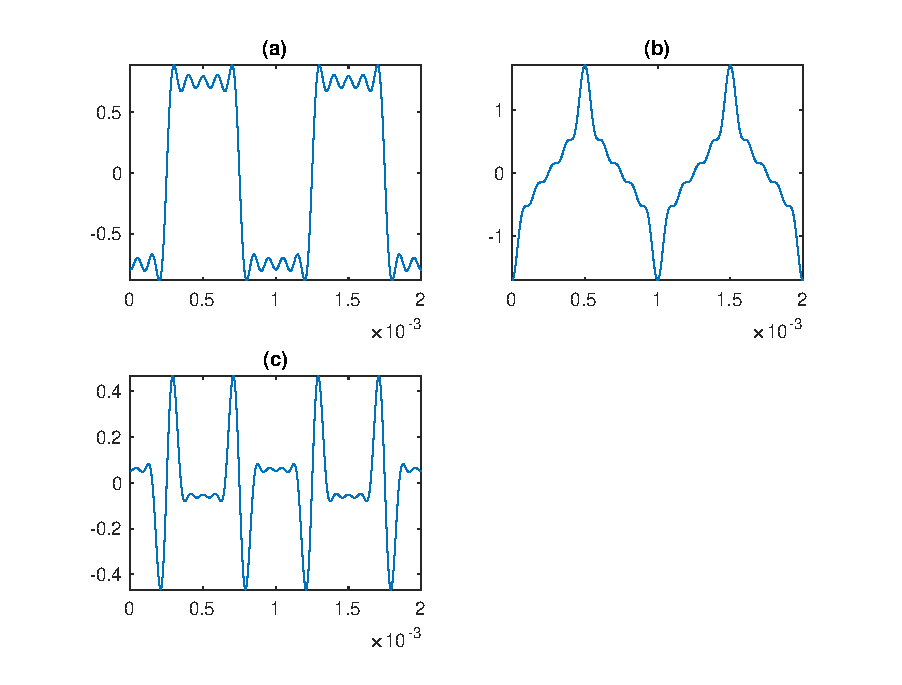
\includegraphics [width=\textwidth]{matlab/fig/D_r_4.eps}
  \caption{waveforms output from filters (a), (b), and (c) after inputting an ideal square wave}    
  \label{fig:D_r_4}
\end{figure}

\begin{tcolorbox}
  D.5) What is the fundamental frequency of the output from filter (c)? Why?
\end{tcolorbox}

3kHz. By definition, the fundamental frequency is the lowest frequency of a Fourier series. The filter zeros out the 1kHz hamonic which is the fundamental frequency of the original signal but keeps the 3kHz hamonic. After this process, the lowest frequency becomes 3kHz for output signal.

\pagebreak